\باب{ترتیب اور تسلسل}
اس باب میں مخلوط اور حقیقی ترتیب اور تسلسل کے بنیادی تصورات پیش کیے جائیں گے۔

\حصہ{ترتیب}\شناخت{حصہ_ترتیب_ترتیب}
تسلسل، بالخصوص طاقتی تسلسل مخلوط تجزیہ میں کلیدی کردار ادا کرتے ہیں۔ان کو متعارف کرنے کی خاطر ہم پہلے ترتیب اور اس سے متعلقہ تصورات کی تعریف پیش کرتے ہیں۔ہم دیکھیں گے کہ مخلوط  ترتیب اور تسلسل کی زیادہ تر مسئلے اور تعریف، حقیقی ترتیب اور تسلسل کے مسائل اور تعریف کی مانند ہوں گے جنہیں حقیقی علم الاحصاء میں استعمال کیا جاتا ہے۔

اگر ہر مثبت عدد صحیح \عددی{n} کو عدد \عددی{z_n} مختص کی جائے تب  ہم کہتے ہیں کہ اعداد
\begin{align*}
z_1,\,z_2,\cdots,z_n,\cdots
\end{align*} 
\اصطلاح{لامتناہی ترتیب}\فرہنگ{ترتیب!لامتناہی}\حاشیہب{infinite sequence}\فرہنگ{sequence} یا،  مختصراً، \اصطلاح{ترتیب} بناتے ہیں۔ان  اعداد \عددی{z_n} کو ترتیب کے \اصطلاح{مقدار} یا  \اصطلاح{اجزاء}\فرہنگ{اجزاء}\حاشیہب{terms}\فرہنگ{terms} کہتے ہیں۔

حقیقی اجزاء پر مبنی ترتیب کو \اصطلاح{حقیقی ترتیب}\فرہنگ{ترتیب!حقیقی}\فرہنگ{حقیقی!ترتیب}\حاشیہب{real sequence}\فرہنگ{real!sequence}\فرہنگ{sequence!real} کہتے ہیں۔

بعض اوقات ہم ترتیب کے اجزاء کی گنتی \عددی{0} یا \عددی{2} یا کسی دیگر عدد صحیح سے شروع کرتے ہیں۔

ایک ترتیب \عددی{z_1,z_2,\cdots} اس صورت \ترچھا{مرکوز}\فرہنگ{مرکوز}  یا \ترچھا{مرتکز}\فرہنگ{مرتکز} ہو گا جب ایسا عدد \عددی{c} پایا جاتا ہو کہ کسی بھی مثبت  (غیر صفر) حقیقی عدد \عددی{\epsilon} (جو چاہے جتنا چھوٹا کیوں نہ ہو) کی صورت میں ہم ایسا عدد صحیح \عددی{N} تلاش کر سکتے ہوں کہ  تمام \عددی{n>N} کے لئے درج ذیل درست ہو۔
\begin{align}\label{مساوات_ترتیب_حد_الف}
\abs{z_n-c}<\epsilon \quad \quad  n>N
\end{align}
\عددی{c} کو ترتیب کی \اصطلاح{حد}\فرہنگ{حد}\حاشیہب{limit}\فرہنگ{limit} کہتے ہیں جس کو عموماً
\begin{align*}
z_n\to c\quad\quad (n\to \infty)
\end{align*}
لکھا جاتا ہے اور ہم کہتے ہیں کہ ترتیب \عددی{c} کو مرکوز ہے یا کہ ترتیب کی حد \عددی{c} ہے۔

ایسا ترتیب جو مرتکز نہ ہو \اصطلاح{منفرج}\فرہنگ{منفرج}\حاشیہب{divergent}\فرہنگ{divergent} کہلاتا ہے۔

مساوات \حوالہ{مساوات_ترتیب_حد_الف} کا  ایک سادہ جیومیٹریائی مطلب ہے۔یہ مساوات کہتی ہے  کہ \عددی{n>N} کی صورت میں ہر جزو \عددی{z_n} اس کھلے قرص میں پایا جاتا ہے جس کا رداس \عددی{\epsilon} اور مرکز \عددی{c} ہے (شکل \حوالہ{شکل_ترتیب_مخلوط_مرتکز})  جبکہ قرص کا رداس \عددی{\epsilon} کتنا ہی کم کیوں نہ کر دیا جائے  اس قرص کے باہر  اجزاء \عددی{z_n} کی زیادہ سے زیادہ تعداد محدود ہو گی۔ظاہر ہے کہ \عددی{N} کی قیمت عموماً \عددی{\epsilon} پر منحصر ہو گی۔
\begin{figure}
\centering
\begin{tikzpicture}
%\draw[thick] (0,0) grid (3,2);
%\draw[thin,gray,step=0.1](0,0) grid (3,2);
%
\draw(0,0)--(3,0)node[right]{$x$};
\draw(0,0)--(0,2)node[left]{$y$};
\foreach \x/\y in {0.1/2,0.2/1.9,0.4/1.8}{\draw[fill](\x,\y)circle (1pt);}
\foreach \x/\y in {0.55/1.85,0.7/1.7,0.9/1.5,1/1.5}{\draw[fill](\x,\y)circle (1pt);}
\foreach \x/\y in {1.05/1.45,1.2/1.35,1.3/1.3,1.3/1.2,1.35/1.2,1.4/1.2}{\draw[fill](\x,\y)circle (1pt);}
\foreach \x/\y in {1.4/1.15,1.5/1.05,1.45/1.15,1.5/1.1}{\draw[fill](\x,\y)circle (1pt);}
\draw(1.5,1)circle (0.75);
\draw[-latex](1.5,1)node[ocirc]{}node[below]{$c$}--++(30:0.75)node[pos=0.35,above]{$\epsilon$};
\end{tikzpicture}
\caption{مرتکز مخلوط ترتیب}
\label{شکل_ترتیب_مخلوط_مرتکز}
\end{figure} 

حقیقی ترتیب کی صورت میں مساوات \حوالہ{مساوات_ترتیب_حد_الف} جیومیٹریائی طور کہتی ہے کہ \عددی{n>N} کی صورت میں جزو \عددی{z_n} وقفہ \عددی{c-\epsilon} تا \عددی{c+\epsilon} پر پایا جائے گا (شکل \حوالہ{شکل_ترتیب_حقیقی_مرتکز}) اور اس وقفہ سے باہر اجزاء کی زیادہ سے زیادہ تعداد محدود ہو گی۔ 
\begin{figure}
\centering
\begin{tikzpicture}
\draw(-2.5,0)--(2.5,0)node[right]{$x$};
\draw(-1.5,0)node[below]{$c-\epsilon$}--++(0,0.1);
\draw(0,0)node[below]{$c$}--++(0,0.1);
\draw(1.5,0)node[below]{$c+\epsilon$}--++(0,0.1);
\end{tikzpicture}
\caption{حقیقی مرتکز ترتیب}
\label{شکل_ترتیب_حقیقی_مرتکز}
\end{figure}

%=======================
\ابتدا{مثال}\شناخت{مثال_ترتیب_مرتکز_اور_منفرج_ترتیب}\quad \موٹا{مرتکز اور منفرج ترتیب}\\
ترتیب \عددی{z_n=1+\tfrac{2}{n}} کے اجزاء 
$3,2,\tfrac{5}{3},\tfrac{6}{4},\tfrac{7}{5},\cdots$
ہیں۔یہ ترتیب  مرتکز ہے اور اس کی حد \عددی{c=1} ہے۔در حقیقت مساوات \حوالہ{مساوات_ترتیب_حد_الف} سے
\begin{align*}
z_n-c=1+\tfrac{2}{n}-1=\tfrac{2}{n}
\end{align*}
لکھا جا سکتا ہے۔یوں \عددی{\tfrac{2}{n}<\epsilon} اس صورت ہو گا جب \عددی{\tfrac{n}{2}>\tfrac{1}{\epsilon}} یا \عددی{n>\tfrac{2}{\epsilon}} ہو۔مثلاً \عددی{\epsilon=0.01} منتخب کرتے ہوئے \عددی{\tfrac{2}{n}<0.01} تب ہو گا جب \عددی{n>200} ہو۔

ترتیب
$1,2,3,\cdots$
اور
$\tfrac{1}{4},\tfrac{3}{4},\tfrac{1}{5},\tfrac{4}{5},\tfrac{1}{6},\tfrac{5}{6},\cdots$
منفرج ہیں۔

وہ ترتیب جس کے اجزاء 
\begin{align*}
z_n=2-\frac{1}{n}+i\big(1+\frac{2}{n}\big)
\end{align*}
یعنی
\begin{align*}
1+i,\quad \frac{3}{2}+i2,\quad \frac{7}{4}+i\frac{3}{2},\cdots
\end{align*}
ہیں کو شکل میں دکھایا گیا ہے۔یہ ترتیب مرتکز ہے اور اس کی حد \عددی{c=2+i} ہے۔مساوات \حوالہ{مساوات_ترتیب_حد_الف} سے
\begin{align*}
\abs{z_n-c}=\abs{\frac{2n-1}{n}+i\frac{n+2}{n}-(2+i)}=\abs{-\frac{1}{n}+i\frac{2}{n}}=\frac{\sqrt{5}}{n}
\end{align*}
لکھا جا سکتا ہے۔یوں \عددی{\tfrac{\sqrt{5}}{n}<\epsilon} تب ہو گا جب \عددی{\tfrac{n}{\sqrt{5}}>\tfrac{1}{\epsilon}} یعنی \عددی{n>\tfrac{\sqrt{5}}{\epsilon}} ہو۔مثال کے طور پر \عددی{\epsilon=\tfrac{1}{100}} منتخب کرتے ہوئے  \عددی{\abs{z_n-c}<\epsilon} تب ہو گا جب \عددی{n>223.6} یعنی
\عددی{n=224} یا \عددی{n=225}، وغیرہ ہو۔
\begin{figure}
\centering
\begin{tikzpicture}
\draw(0,0)--(3,0)node[right]{$x$};
\draw(0,0)--(0,3.5)node[right]{$y$};
\foreach \x in {1,2}{\draw(\x,0)node[below]{$\x$}--++(0,0.1);}
\foreach \y in {1,2,3}{\draw(0,\y)node[left]{$\y$}--++(0.1,0);}
\foreach \n in {1,2,3,4,5,6,7,8,9,10,11,12,16,20,25,30,40,60,80,90,100}{\draw[fill](2-1/\n,1+2/\n) circle (1pt);}
\draw(2,1)node[ocirc]{}node[right]{$c=2+i$};
\draw(0,0)node[below]{$0$}node[left]{$0$};
\end{tikzpicture}
\caption{مثال \حوالہ{مثال_ترتیب_مرتکز_اور_منفرج_ترتیب} میں آخری ترتیب}
\label{شکل_مثال_ترتیب_مرتکز_اور_منفرج_ترتیب}
\end{figure}
\انتہا{مثال}
%===========================
مخلوط ترتیب \عددی{z_1,z_2,z_3,\cdots} کی صورت میں \عددی{z_n=x_n+iy_n} لکھ کر ہم حقیقی حصوں کی ترتیب اور خیالی حصوں کی ترتیب
\begin{align*}
x_1,x_2,x_3,\cdots\quad \text{اور}\quad y_1,y_2,y_3,\cdots
\end{align*}
 پر علیحدہ علیحدہ غور کر سکتے ہیں۔مثلاً  مثال \حوالہ{مثال_ترتیب_مرتکز_اور_منفرج_ترتیب} کی آخری ترتیب کے دو علیحدہ علیحدہ ترتیب درج ذیل ہوں گی۔
\begin{align*}
1,\frac{3}{2},\frac{5}{3},\frac{7}{4},\cdots \quad \text{اور}\quad 3,2,\frac{5}{3},\frac{3}{2},\cdots
\end{align*}
ہم دیکھتے ہیں کہ حقیقی اور خیالی ترتیب کے حد  بالترتیب \عددی{2} اور \عددی{1} ہیں (شکل \حوالہ{شکل_مثال_ترتیب_مرتکز_اور_منفرج_ترتیب}) جو اصل مخلوط ترتیب کی حقیقی اور خیالی حصوں کی حد ہیں۔عموماً ایسا ہی ہوتا ہے جو درج ذیل کی ایک مثال ہے۔ 

%==================
\ابتدا{مسئلہ}\شناخت{مسئلہ_ترتیب_حقیقی_خیالی_اجزاء_ترتیب}\quad \موٹا{(حقیقی اور خیالی اجزاء کی ترتیب)}\\
مخلوط اعداد \عددی{z_n=x_n+iy_n\quad (n=1,2,\cdots)} کی ترتیب \عددی{z_1,z_2,\cdots,z_n,\cdots} صرف اور صرف اس صورت حد \عددی{c=a+ib} پر مرکوز ہو گا جب حقیقی حصوں کی ترتیب   \عددی{x_1,x_2,\cdots} نقطہ \عددی{a} پر مرتکز ہو اور خیالی حصوں کی ترتیب \عددی{y_1,y_2,\cdots} نقطہ \عددی{b} پر مرتکز ہو۔
\انتہا{مسئلہ}
%=======================
\ابتدا{ثبوت}\quad
اگر \عددی{\abs{z_n-c}<\epsilon} ہو تب  \عددی{z_n=x_n+iy_n} اس دائرہ کے اندر پایا جائے گا جس کا رداس \عددی{\epsilon} اور مرکز \عددی{c=a+ib} ہوں۔ یوں لازماً 
\begin{align*}
\abs{x_n-a}<\epsilon, \quad \abs{y_n-b}<\epsilon
\end{align*}
ہو گا (شکل \حوالہ{شکل_مسئلہ_ترتیب_حقیقی_خیالی_اجزاء_ترتیب}-الف)۔ یوں \عددی{n\to \infty} کی صورت میں مرکوزیت \عددی{z_n\to c} سے مراد مرکوزیت \عددی{x_n\to a} اور مرکوزیت \عددی{y_n\to b} ہے۔
\begin{figure}
\centering
\begin{subfigure}{0.5\textwidth}
\centering
\begin{tikzpicture}
\pgfmathsetmacro{\xlen}{1.5}
\pgfmathsetmacro{\ylen}{1.5}
\pgfmathsetmacro{\r}{1}
\draw(\xlen,\ylen)coordinate(kA);
%
\draw(0,0)--(3.5,0)node[right]{$x$};
\draw(0,0)--(0,3)node[right]{$y$};
%
\draw[dashed](kA)--(\xlen,0)node[below]{$a$};
\draw[dashed](kA)--(0,\ylen)node[left]{$b$};
\draw[dashed](\xlen,\ylen+\r)--(0,\ylen+\r)node[left]{$b+\epsilon$};
\draw[dashed](\xlen,\ylen-\r)--(0,\ylen-\r)node[left]{$b-\epsilon$};
\draw[dashed](\xlen-\r,\ylen)--(\xlen-\r,0)node[below]{$a-\epsilon$};
\draw[dashed](\xlen+\r,\ylen)--(\xlen+\r,0)node[below]{$a+\epsilon$};
\draw(kA)node[ocirc]{}node[right]{$c$} circle (\r);
\end{tikzpicture}
\caption*{(الف)}
\end{subfigure}%
\begin{subfigure}{0.5\textwidth}
\centering
\begin{tikzpicture}
\pgfmathsetmacro{\xlen}{1.5}
\pgfmathsetmacro{\ylen}{1.5}
\pgfmathsetmacro{\r}{1}
\draw(\xlen,\ylen)coordinate(kA);
%
\draw(0,0)--(3.5,0)node[right]{$x$};
\draw(0,0)--(0,3)node[right]{$y$};
%
\draw[dashed](kA)--(\xlen,0)node[below]{$a$};
\draw[dashed](kA)--(0,\ylen)node[left]{$b$};
\draw[dashed](\xlen-\r/2,\ylen+\r/2)--(0,\ylen+\r/2)node[left]{$b+\tfrac{\epsilon}{2}$};
\draw[dashed](\xlen-\r/2,\ylen-\r/2)--(0,\ylen-\r/2)node[left]{$b-\tfrac{\epsilon}{2}$};
\draw[dashed](\xlen-\r/2,\ylen-\r/2)--(\xlen-\r/2,0);
\draw[dashed](\xlen+\r/2,\ylen-\r/2)--(\xlen+\r/2,0);
\draw(kA)node[ocirc]{}node[right]{$c$} circle (\r);
\draw[thick](\xlen-\r/2,\ylen-\r/2) rectangle ++(\r,\r);
\draw[stealth-](\xlen-\r/2,0)++(0,-0.1) to [out=-90,in=0]++(-0.3,-0.3)node[left]{$a-\tfrac{\epsilon}{2}$};
\draw[stealth-](\xlen+\r/2,0)++(0,-0.1) to [out=-90,in=180]++(0.3,-0.3)node[right]{$a+\tfrac{\epsilon}{2}$};
\end{tikzpicture}
\caption*{(ب)}
\end{subfigure}%
\caption{مسئلہ \حوالہ{مسئلہ_ترتیب_حقیقی_خیالی_اجزاء_ترتیب} کا ثبوت}
\label{شکل_مسئلہ_ترتیب_حقیقی_خیالی_اجزاء_ترتیب}
\end{figure}

اس کی الٹ چلتے ہوئے، اگر \عددی{n\to \infty} کی صورت میں \عددی{x_n\to a} اور \عددی{y_n\to b} ہوں  تب کسی بھی دیے گئے \عددی{\epsilon>0} کی صورت میں ہم ایسا \عددی{N} اتنا بڑا منتخب کر سکتے ہیں کہ ہر \عددی{n>N} کے لئے 
\begin{align*}
\abs{x_n-a}<\frac{\epsilon}{2},\quad \abs{y_n-b}<\frac{\epsilon}{2}
\end{align*}
ہو۔ان دو عدم مساوات کہتی ہیں کہ \عددی{z_n=x_n+iy_n} اس چکور کے اندر پایا جائے گا جس کے اطراف کی لمبائی \عددی{\epsilon} اور مرکز \عددی{c} ہو (شکل \حوالہ{شکل_مسئلہ_ترتیب_حقیقی_خیالی_اجزاء_ترتیب}-ب)۔یوں ثبوت مکمل ہوتا ہے۔
\انتہا{ثبوت}
%=================

اس مسئلہ کی باعث حقیقی حصہ اور خیالی حصہ کی ترتیب پر غور کرتے ہوئے مخلوط ترتیب کی مرکوزیت کو حقیقی ترتیب سے حاصل کیا جا سکتا ہے۔

اگر ایسا مثبت عدد \عددی{K} پایا جاتا ہو کہ مرکز پر رداس \عددی{K} کے دائرے میں ترتیب \عددی{z_1,z_2,\cdots} کے تمام اجزاء  پائے جاتے ہوں  یعنی
\begin{align*}
\abs{z_n}<K \quad \quad \text{\RL{تمام $n$}}
\end{align*}
تب یہ ترتیب \اصطلاح{محدود}\فرہنگ{محدود}\حاشیہب{bounded}\فرہنگ{bounded} کہلاتا  ہے۔ایسا ترتیب جو محدود نہ ہو \اصطلاح{غیر محدود}\فرہنگ{غیر محدود}\حاشیہب{unbounded}\فرہنگ{unbounded} کہلاتا ہے۔

اس تصور کو استعمال کرتے ہوئے انفراج  کو عموماً درج ذیل سادہ مسئلہ  سے دریافت کیا جا سکتا ہے۔

%=========================
\ابتدا{مسئلہ}\شناخت{مسئلہ_ترتیب_مرتکز_ترتیب_محدود_ہو_گی}
ہر مرتکز ترتیب محدود ہو گی۔یوں اگر ایک ترتیب غیر محدود ہو تب یہ منفرج ہو گی۔
\انتہا{مسئلہ}
%===========================
\ابتدا{ثبوت}
فرض کریں کہ ترتیب \عددی{z_1,z_2,\cdots} مرکوز ہے اور اس کی حد \عددی{c} ہے۔ تب ہم \عددی{\epsilon>0} منتخب کرتے ہوئے ایسا مطابقتی \عددی{N} تلاش کر سکتے ہیں کہ  \عددی{n>N} کے لئے ہر \عددی{z_n} رداس \عددی{\epsilon} کے قرص، جس کا مرکز \عددی{c} ہو، میں پائے جائیں گے اور وہ  \عددی{z_n} جو اس قرص کے باہر ہوں کی زیادہ سے زیادہ تعداد محدود ہو گی۔اب ظاہر ہے کہ ہم مرکز پر اتنے بڑی  رداس \عددی{K} کا دائرہ منتخب کر سکتے ہیں کہ یہ قرص اور قرص کے باہر تمام \عددی{z_n} اس دائرے میں پائیں جاتے ہوں۔اس سے ثابت ہوتا ہے کہ یہ ترتیب محدود ہے۔
\انتہا{ثبوت}
%=========================

یہاں دہان رہے کہ محدود ہونا مرکوزیت کے لئے کافی نہیں ہے۔مثلاً ترتیب \عددی{1,0,1,0,\cdots} محدود  لیکن منفرج ہے۔ (کیوں؟) غیر محدود ترتیب کی مثالیں درج ذیل ہیں
\begin{align*}
1,2,3,4,\cdots\quad \text{اور}\quad \frac{1}{2},2,\frac{1}{3},3,\frac{1}{4},4,\cdots
\end{align*} 
جو مسئلہ \حوالہ{مسئلہ_ترتیب_مرتکز_ترتیب_محدود_ہو_گی} کے تحت منفرج ترتیب ہیں۔

%=====================
\حصہء{سوالات}
سوال \حوالہ{سوال_ترتیب_نقشہ_الف} تا سوال \حوالہ{سوال_ترتیب_نقشہ_ب} میں دیے ترتیب کے ابتدائی چند اجزاء لکھ کر ترسیم کریں۔

%======================
\ابتدا{سوال}\شناخت{سوال_ترتیب_نقشہ_الف}\quad
$\tfrac{n}{n+3}$\\
جواب:\quad
$\tfrac{1}{4},\tfrac{2}{5},\tfrac{1}{2},\tfrac{4}{7},\tfrac{5}{8},\cdots$
\انتہا{سوال}
%======================
\ابتدا{سوال}\quad
$\tfrac{2n}{n^2+1}$\\
جواب:\quad
$1,\tfrac{4}{5},\tfrac{3}{5},\tfrac{8}{17},\tfrac{5}{13},\cdots$
\انتہا{سوال}
%======================
\ابتدا{سوال}\شناخت{سوال_ترتیب_نقشہ_پ}\quad
$\tfrac{i^n}{n^2}$\\
جواب:\quad
$i,-\tfrac{1}{4},-\tfrac{i}{9},\tfrac{1}{16},\tfrac{i}{25},\cdots$
\انتہا{سوال}
%======================
\ابتدا{سوال}\quad
$\tfrac{in}{n+1}$\\
جواب:\quad
$\tfrac{i}{2},\tfrac{i2}{3},\tfrac{i3}{4},\tfrac{i4}{5},\tfrac{i5}{6},\cdots$
\انتہا{سوال}
%======================
\ابتدا{سوال}\quad
$\tfrac{i^n n^2}{n+i}$\\
جواب:\quad
$\tfrac{1}{2}(1+i),\tfrac{4}{5}(-2+i),\tfrac{9}{10}(-1-i3),\tfrac{16}{17}(4-i),\tfrac{25}{26}(1+i5),\cdots$
\انتہا{سوال}
%======================
\ابتدا{سوال}\شناخت{سوال_ترتیب_نقشہ_ب}\quad
$(-1)^n+i2\pi n$\\
جواب:\quad
$-1+i2\pi, 1+i4\pi,-1+i6\pi, 1+i8\pi, -1+i10\pi,\cdots$
\انتہا{سوال}
%======================
\ابتدا{سوال}\quad
ترتیب \عددی{z_1=1}، \عددی{z_2=\tfrac{i}{2}}، \عددی{z_n=iz_{n-2}z_{n-1}\,\, (n=3,4,\cdots)} کے ابتدائی چند اجزاء لکھیں۔اس ترتیب  کی حد تلاش کریں۔\\
جواب:\quad
$1,\tfrac{i}{2}, -\tfrac{1}{2},\tfrac{1}{4}, -\tfrac{i}{8},\cdots$
\انتہا{سوال}
%=========================
سوال \حوالہ{سوال_ترتیب_محدود_مرکوز_حد_الف} تا سوال \حوالہ{سوال_ترتیب_محدود_مرکوز_حد_ب} میں دریافت کریں کہ آیا دی گئی ترتیب محدود ہے؟ کیا یہ ترتیب مرکوز ہے؟ مرکوزیت کی صورت میں ترتیب کی حد تلاش کریں۔
  
%================
\ابتدا{سوال}\شناخت{سوال_ترتیب_محدود_مرکوز_حد_الف}\quad
$z_n=i^n$\\
جواب:\quad
محدود، منفرج
\انتہا{سوال}
%======================
\ابتدا{سوال}\quad
$z_n=\tfrac{i^n}{n}$\\
جواب:\quad
محدود، مرکوز، حد $0$
\انتہا{سوال}
%======================
\ابتدا{سوال}\quad
$z_n=\tfrac{in}{n+1}$\\
جواب:\quad
محدود، مرکوز، حد $i$
\انتہا{سوال}
%======================
\ابتدا{سوال}\quad
$z_n=\tfrac{n^2}{n+i}$\\
جواب:\quad
غیر محدود، منفرج
\انتہا{سوال}
%======================
\ابتدا{سوال}\quad
$z_n=\tfrac{(-1)^n}{n^3}$\\
جواب:\quad
محدود، مرکوز، حد $0$
\انتہا{سوال}
%======================
\ابتدا{سوال}\شناخت{سوال_ترتیب_محدود_مرکوز_حد_ب}\quad
$z_n=e^{i\tfrac{n\pi}{4}}$\\
جواب:\quad
محدود، منفرج
\انتہا{سوال}
%======================
\ابتدا{سوال}\quad \موٹا{حد کی یکتائی}\\
دکھائیں کہ اگر ایک ترتیب مرتکز ہو تب اس کا حد یکتا ہو گا۔
\انتہا{سوال}
%=========================
\ابتدا{سوال}\quad
ثابت کریں (مثال \حوالہ{مثال_ترتیب_مرتکز_اور_منفرج_ترتیب} کی طرح) کہ 
$\tfrac{i^n}{n^3}$
مرکوز ہے۔
\انتہا{سوال}
%============================
\ابتدا{سوال}\quad
ایک ترتیب کے اجزاء درج ذیل کلیہ دیتی ہے۔اس ترتیب کو استعمال کرتے ہوئے مسئلہ \حوالہ{مسئلہ_ترتیب_حقیقی_خیالی_اجزاء_ترتیب} کی تصدیق کریں۔\\
\begin{align*}
z_n=\frac{n^2-1}{2n^2+1}+i\frac{n}{n+2}
\end{align*}
\انتہا{سوال}
%====================
\ابتدا{سوال}\quad
دکھائیں کہ مخلوط ترتیب \عددی{z_1,z_2,\cdots} اس صورت محدود ہو گی جب اس کے حقیقی حصہ اور خیالی حصہ کے مطابقتی ترتیب محدود ہوں۔
\انتہا{سوال}
%====================
\ابتدا{سوال}\quad
اگر ترتیب \عددی{z_1,z_2,\cdots} مرکوز ہو اور اس کا حد \عددی{0} ہو، اور ترتیب \عددی{b_1,b_2,\cdots} کسی مقررہ \عددی{K>0} اور تمام \عددی{n} کے  لئے  \عددی{\abs{b_n}\le K\abs{z_n}} کو مطمئن کرتا ہو تب دکھائیں کہ ترتیب \عددی{b_1,b_2,\cdots} مرکوز ہے اور اس کا حد \عددی{0} ہے۔
\انتہا{سوال}
%========================
\ابتدا{سوال}\شناخت{سوال_ترتیب_مجموعہ_کا_حد}\quad
اگر ترتیب \عددی{z_1,z_2,\cdots} مرکوز ہو اور اس کا حد \عددی{l} ہو اور ترتیب \عددی{z^*_1,z^*_2,\cdots} مرکوز ہو اور اس کا حد \عددی{l^*}  ہو تب دکھائیں کہ ترتیب \عددی{z_1+z^*_1,z_2+z^*_2,\cdots} مرکوز ہو گا اور اس کا حد \عددی{l+l^*} ہو گا۔
\انتہا{سوال}
%=========================
\ابتدا{سوال}\quad
سوال \حوالہ{سوال_ترتیب_مجموعہ_کا_حد} کے مفروضوں کے ساتھ دکھائیں کہ ترتیب \عددی{z_1z^*_1,z_2z^*_2,\cdots}  مرکوز ہو گا اور اس کا حد \عددی{ll^*} ہو گا۔
\انتہا{سوال}
%========================

\حصہ{تسلسل}
فرض کریں کہ \عددی{w_1,w_2,\cdots,w_m,\cdots} حقیقی یا مخلوط اعداد کی ترتیب ہے۔تب ہم درج ذیل \ترچھا{لامتناہی تسلسل} یا، مختصراً، \اصطلاح{تسلسل}\فرہنگ{تسلسل}\حاشیہب{series}\فرہنگ{series} پر غور کرتے ہیں۔
\begin{align}\label{مساوات_ترتیب_تسلسل_الف}
\sum_{m=1}^{\infty} w_m=w_1+w_2+w_3+\cdots
\end{align}
\عددی{w_m} کو ترتیب کی \ترچھا{مقدار} یا  \اصطلاح{اجزاء}\فرہنگ{اجزاء}\حاشیہب{terms}\فرہنگ{terms} کہتے ہیں۔ابتدائی \عددی{n} اجزاء کے مجموعہ
\begin{align}\label{مساوات_ترتیب_تسلسل_ب}
s_n=w_1+w_2+\cdots+w_n
\end{align}
کو تسلسل \حوالہ{مساوات_ترتیب_تسلسل_الف} کا \عددی{n} واں \اصطلاح{جزوی مجموعہ}\فرہنگ{جزوی مجموعہ}\فرہنگ{مجموعہ!جزوی}\حاشیہب{partial sum}\فرہنگ{sum!partial} کہتے ہیں۔ تسلسل \حوالہ{مساوات_ترتیب_تسلسل_الف} سے  \عددی{s_n} ترک کرنے سے
\begin{align}
R_n=w_{n+1}+w_{n+2}+w_{n+3}+\cdots
\end{align}
باقی رہ جاتا ہے جس کو تسلسل \حوالہ{مساوات_ترتیب_تسلسل_الف} کا، \عددی{n} اجزاء کے بعد، \اصطلاح{باقی}\فرہنگ{باقی}\حاشیہب{remainder}\فرہنگ{remainder} کہتے ہیں۔ 

اس طرح ہم تسلسل \حوالہ{مساوات_ترتیب_تسلسل_الف} کے ساتھ اس کے جزوی مجموعوں \عددی{s_1,s_2,s_3,\cdots} کی ترتیب وابستہ کرتے ہیں۔اگر یہ ترتیب مرتکز ہو، مثلاً،
\begin{align*}
\lim_{n\to \infty} s_n=s
\end{align*}
تب ہم کہتے ہیں کہ تسلسل \حوالہ{مساوات_ترتیب_تسلسل_الف} \اصطلاح{مرکوز}\فرہنگ{مرکوز}\حاشیہب{convergent}\فرہنگ{convergent} یا \اصطلاح{مرتکز} ہے اور عدد \عددی{s} اس کی \اصطلاح{قیمت}\فرہنگ{قیمت}\حاشیہب{value}\فرہنگ{value} یا \ترچھا{مجموعہ}\فرہنگ{مجموعہ} کہلاتا ہے اور ہم درج ذیل لکھتے ہیں۔
\begin{align*}
s=\sum_{m=1}^{\infty} w_m=w_1+w_2+w_3+\cdots
\end{align*}

اگر جزوی مجموعوں کی ترتیب منفرج ہو تب ہم کہتے ہیں کہ تسلسل  \حوالہ{مساوات_ترتیب_تسلسل_الف}  \اصطلاح{منفرج}\فرہنگ{منفرج}\حاشیہب{divergent}\فرہنگ{divergent} ہے۔

اگر تسلسل \حوالہ{مساوات_ترتیب_تسلسل_الف} مرکوز ہو اور اس کی قیمت \عددی{s} ہو تب
\begin{align}
s=s_n+R_n\quad \implies \quad R_n=s-s_n
\end{align}
ہو گا۔مرکوزیت کی تعریف کے تحت \عددی{n} کو کافی بڑا لیتے ہوئے  ہم \عددی{\abs{R_n}} کو جتنا چاہیں چھوٹا بنا سکتے ہیں۔ بہت سی صورتوں میں مرکوز تسلسل کا مجموعہ \عددی{s} تلاش کرنا نا ممکن ہو گا۔تب حساب کی خاطر ہم اس کے جزوی مجموعہ \عددی{s_n} کو \عددی{s} کی تقریب تصور کریں گے اور \عددی{R_n} کا تخمینہ لگا کر  تقریب کی درستگی کا جائزہ لیں گے۔

%===================
\ابتدا{مثال}\شناخت{مثال_ترتیب_ہارمونی_منفرج}\quad \موٹا{مرتکز اور منفرج تسلسل}\\
تسلسل
\begin{align*}
\sum_{m=1}^{\infty} \frac{1}{2^m}=\frac{1}{2}+\frac{1}{4}+\frac{1}{8}+\cdots
\end{align*}
مرکوز ہے اور چونکہ
\begin{align*}
s_n=\frac{1}{2}+\frac{1}{4}+\frac{1}{8}+\cdots+\frac{1}{2^n}=1-\frac{1}{2^n} \quad \implies\quad  \lim_{n\to \infty}s_n=1
\end{align*}
ہے لہٰذا تسلسل کی قیمت \عددی{1} ہے۔اس کے برعکس تسلسل
\begin{align*}
\sum_{m=1}^{\infty} m=1+2+3+\cdots
\end{align*}
منفرج ہے اور تسلسل
\begin{align*}
\sum_{m=0}^{\infty} (-1)^m=1-1+1-+\cdots
\end{align*}
منفرج ہے چونکہ 
\begin{align*}
s_0=1, \quad s_1=1-1=0,\quad s_2=1-1+1=1, \cdots
\end{align*}
ہے  اور ترتیب \عددی{1,0,1,0,\cdots} منفرج ہے۔

\اصطلاح{ہارمونی تسلسل}\فرہنگ{ہارمونی!تسلسل}\حاشیہب{harmonic series}\فرہنگ{harmonic!series}
\begin{align*}
\sum_{m=1}^{\infty} \frac{1}{m}=1+\frac{1}{2}+\frac{1}{3}+\cdots
\end{align*}
منفرج ہے۔در حقیقت جزوی مجموعہ \عددی{s_n}
\begin{align*}
s_n=1+\frac{1}{2}+\cdots+\frac{1}{n}
\end{align*}
شکل \حوالہ{مثال_ترتیب_ہارمونی_منفرج} میں \عددی{n} عدد مستطیل کے نیچے رقبہ کے برابر ہے۔یہ رقبہ قوس \عددی{y=\tfrac{1}{x}} کے نیچے مطابقتی رقبہ \عددی{A_n} سے زیادہ ہے۔اب 
\begin{align*}
A_n=\int_1^{n+1}\frac{\dif x}{x}=\ln(n+1)\to \infty \quad \quad (n\to \infty)
\end{align*}
ہے اور چونکہ \عددی{s_n>A_n} ہے لہٰذا \عددی{n\to \infty} کرنے سے \عددی{s_n\to\infty} حاصل ہو گا جو انفراج کی تعریف ہے۔
\begin{figure}
\centering
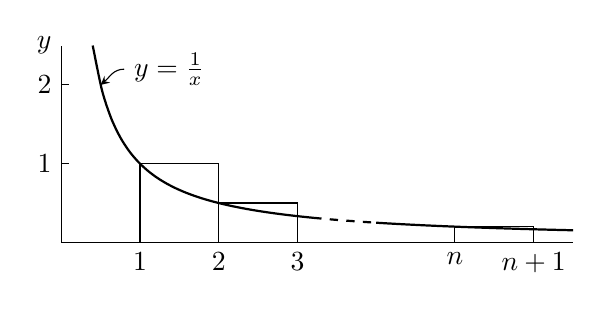
\begin{tikzpicture}
\draw(0,0)--(6.5,0);
\draw(0,0)--(0,2.5)node[left]{$y$};
\foreach \x in {1,2,3}{\draw(\x,0)node[below]{$\x$};}
\foreach \y in {1,2}{\draw(0,\y)node[left]{$\y$}--++(0.1,0);}
\draw[thick,domain=0.4:3.2,variable=\x,smooth]  plot ({\x},{1/\x});
\draw[thick,dashed,domain=3.2:4,variable=\x,smooth]  plot ({\x},{1/\x});
\draw[thick,domain=4:6.5,variable=\x,smooth]  plot ({\x},{1/\x});
\draw(1,0)--++(0,1)--++(1,0)--++(0,-1);
\draw(2,1/2)--++(1,0)--++(0,-1/2);
\draw(5,0)node[below]{$n$}--++(0,0.2)--++(1,0)--++(0,-0.2)node[below]{$n+1$};
\draw[stealth-](0.5,2) to [out=40,in=180]++(0.3,0.2)node[right]{$y=\frac{1}{x}$};
\end{tikzpicture}
\caption{شکل برائے مثال \حوالہ{مثال_ترتیب_ہارمونی_منفرج}}
\label{شکل_مثال_ترتیب_ہارمونی_منفرج}
\end{figure}
\انتہا{مثال}
%========================

مسئلہ \حوالہ{مسئلہ_ترتیب_حقیقی_خیالی_اجزاء_ترتیب} سے  فوری طور پر تسلسل کے لئے درج ذیل مسئلہ حاصل ہوتا ہے۔

%===============
\ابتدا{مسئلہ}\quad \موٹا{حقیقی اور خیالی حصوں کی تسلسل}\\
فرض کریں کہ \عددی{w_m=u_m+iv_m} ہے۔تب تسلسل
\begin{align*}
\sum_{m=1}^{\infty} w_m=w_1+w_2+w_3+\cdots
\end{align*}
کی قیمت صرف اور صرف اس صورت \عددی{s=a+jb} ہو گی جب حقیقی حصہ کی تسلسل اور خیالی حصہ کی تسلسل 
\begin{align*}
\sum_{m=1}^{\infty} u_m=u_1+u_2+u_3+\cdots\quad \text{}\quad \sum_{m=1}^{\infty} v_m=v_1+v_2+v_3+\cdots
\end{align*}
مرکوز ہوں اور حقیقی حصے کی تسلسل کی قیمت \عددی{a} اور خیالی حصے کی تسلسل کی قیمت  \عددی{b} ہو۔
\انتہا{مسئلہ}
%====================== 

یہ مسئلہ حقیقی اور مخلوط تسلسل کے درمیان تعلق دیتا ہے۔اس سے زیادہ اہم تعلق درج ذیل تصور پر مبنی ہے۔ 

تسلسل \عددی{w_1+w_2+\cdots} اس صورت \اصطلاح{حتمی مرتکز}\فرہنگ{مرتکز!حتمی}\حاشیہب{absolutely convergent}\فرہنگ{convergent!absolutely}  کہلاتا ہے جب مطابقتی تسلسل
\begin{align}\label{مساوات_ترتیب_حتمی_مرتکز}
\sum_{m=1}^{\infty} \abs{w_m}=\abs{w_1}+\abs{w_2}+\cdots
\end{align}
(جس کے اجزاء حقیقی اور غیر منفی ہیں) مرتکز ہو۔

اگر تسلسل \عددی{w_1+w_2+\cdots} مرکوز ہو جبکہ  تسلسل \حوالہ{مساوات_ترتیب_حتمی_مرتکز} منفرج ہو تب تسلسل  \اصطلاح{مشروط مرتکز}\فرہنگ{مرتکز!مشروط}\حاشیہب{conditional convergent}\فرہنگ{convergent!conditional}  کہلاتا ہے۔

%====================
\ابتدا{مثال}\quad \موٹا{حتمی اور مشروط مرکوز تسلسل}\\
تسلسل
\begin{align*}
\frac{1}{2}-\frac{1}{4}+\frac{1}{8}-\frac{1}{16}+-\cdots
\end{align*}
حتمی مرتکز ہے چونکہ مطابقتی تسلسل \حوالہ{مساوات_ترتیب_حتمی_مرتکز} مرکوز ہے (مثال \حوالہ{مثال_ترتیب_ہارمونی_منفرج})۔اس کے برعکس تسلسل
\begin{align*}
1-\frac{1}{2}+\frac{1}{3}-\frac{1}{4}+-\cdots
\end{align*}
مشروط مرکوز ہے چونکہ تسلسل از خود (معیار لیبنٹز کے تحت) مرتکز ہے لیکن مطابقتی تسلسل \حوالہ{مساوات_ترتیب_حتمی_مرتکز} ہارمونی ہے جو منفرج ہے (مثال \حوالہ{مثال_ترتیب_ہارمونی_منفرج})۔
\انتہا{مثال}
%===========================

حتمی مرتکز تسلسل کی درج ذیل خاصیت بالکل واضح ہے۔

%=============== 
\ابتدا{مسئلہ}
اگر تسلسل \عددی{w_1+w_2+\cdots} حتمی مرتکز ہو تب یہ مرکوز ہو گا۔
\انتہا{مسئلہ}
%=======================

ہم اگلے حصے کی آخر میں کوشی اصول مرکوزیت کی مدد سے  اس مسئلے کا سادہ ثبوت پیش کریں گے۔

ہم آخر میں ایک سادہ مسئلہ پیش کرتے ہیں جو عموماً کارآمد ثابت ہوتا ہے۔

%=====================
\ابتدا{مسئلہ}
اگر تسلسل \عددی{w_1+w_2+\cdots} مرتکز ہو تب
\begin{align}\label{مساوات_ترتیب_مرکوزیت_شرط}
\lim_{m\to\infty} w_m=0
\end{align}
ہو گا۔یوں وہ تسلسل جو مساوات \حوالہ{مساوات_ترتیب_مرکوزیت_شرط} کو مطمئن نہ کرتا ہو منفرج ہو گا۔
\انتہا{مسئلہ}
%==============================
\ابتدا{ثبوت}\quad
فرض کریں کہ \عددی{w_1+w_2+\cdots} مرتکز ہے اور اس کا مجموعہ \عددی{s} ہے۔ تب 
\begin{align*}
w_{n+1}=s_{n+1}-s_n
\end{align*}
اور
\begin{align*}
\lim_{n\to\infty} (s_{n+1}-s_n)=\lim_{n\to\infty}s_{n+1} -\lim_{n\to\infty}s_n=s-s=0
\end{align*}
ہو گا۔
\انتہا{ثبوت}
%==========================

یاد رہے کہ مساوات \حوالہ{مساوات_ترتیب_مرکوزیت_شرط} مرکوزیت کے لئے لازمی لیکن نا کافی شرط ہے۔ مثلاً مثال \حوالہ{مثال_ترتیب_ہارمونی_منفرج} کی ہارمونی تسلسل مساوات \حوالہ{مساوات_ترتیب_مرکوزیت_شرط} کو مطمئن کرتے ہوئے بھی  منفرج ہے۔  مساوات \حوالہ{مساوات_ترتیب_مرکوزیت_شرط} میں دوسری اور تیسری تسلسل مساوات  \حوالہ{مساوات_ترتیب_مرکوزیت_شرط} کو مطمئن نہیں کرتے ہیں لہٰذا وہ منفرج ہیں۔

%============================
\حصہ{کوشی اصول مرکوزیت برائے ترتیب اور تسلسل}
کسی بھی ترتیب یا تسلسل کو استعمال کرنے سے پہلے ہم جاننا چاہیں گے کہ آیا وہ مرتکز ہے یا نہیں۔چونکہ ہمیں پہلے سے حد معلوم نہیں ہوتا ہے لہٰذا مرکوزیت کی تعریف سے ایسا فیصلہ کرنا عموماً ممکن نہیں ہو گا۔کوشی اصول مرکوزیت سے، حد جانے بغیر مرکوزیت دریافت کرتا ہے۔

کوشی اصول مرکوزیت میں ہم  مسئلہ بُلزانو وائشسٹراس زیر استعمال لائیں گے۔ مسئلہ بُلزانو وائشسٹراس کو بیان کرنے کی خاطر درج ذیل تصور کی ضرورت ہو گی۔  

نقطہ \عددی{a} اس صورت ترتیب \عددی{z_1,z_2,\cdots} کا \اصطلاح{تحدیدی نقطہ}\فرہنگ{تحدیدی!نقطہ}\فرہنگ{نقطہ!تحدیدی}\حاشیہب{limit point}\فرہنگ{limit!point} کہلائے گا جب کسی بھی دیے گئے \عددی{\epsilon>0} (جو جتنا چاہیں چھوٹا کیوں نا ہو)  کے لئے درج ذیل درست ہو۔
\begin{align}\label{مساوات_ترتیب_تحدیدی_نقطہ}
\abs{z_n-a}<\epsilon \quad \quad \text{\RL{(جہاں \عددی{n} لامتناہی تعداد ہے)}}
\end{align}
جیومیٹریائی طور پر اس کا مطلب ہے کہ \عددی{\epsilon} کو جتنا بھی چھوٹا کیوں نہ منتخب کیا جائے، رداس \عددی{\epsilon} کا دائرہ جس کا مرکز \عددی{a} ہو، میں تسلسل کے نقطوں کی لامتناہی تعداد پائی جائے گی۔

دھیان رہے کہ مساوات \حوالہ{مساوات_ترتیب_تحدیدی_نقطہ} مطمئن ہونے کے باوجود  دائرے کے باہر نقطوں کی تعداد لامتناہی ہو سکتی ہے اور ترتیب منفرج ہو سکتا ہے۔ در حقیقت مرتکز ترتیب کا حد ہی تحدیدی نقطہ ہو گا (کیوں؟)  اور یہ ترتیب کا واحد تحدیدی نقطہ ہو گا۔اگر کسی ترتیب کا ایک سے زیادہ تحدیدی نقطہ پایا جاتا ہو تب یہ ترتیب منفرج ہو گا۔

مزید، اگر ایک نقطہ لامتناہی بار کسی ترتیب میں پایا جاتا ہو تب تحدیدی نقطہ کی تعریف کے تحت یہی نقطہ اس ترتیب کا تحدیدی نقطہ ہو گا۔

آئیں صورت حال کو سمجھنے کے لئے مثال \حوالہ{مثال_ترتیب_جدول_تحدیدی_نقطہ_وغیرہ} دیکھتے ہیں۔یاد رہے کہ حصہ \حوالہ{حصہ_ترتیب_ترتیب} کے آخر کے قریب محدود ہونے کی تعریف پیش کی گئی۔

%=========================
\ابتدا{مثال}\شناخت{مثال_ترتیب_جدول_تحدیدی_نقطہ_وغیرہ}\quad \موٹا{تحدیدی نقطہ، مرکوزیت اور محدود ہونا}\\
جدول \حوالہ{جدول_مثال_ترتیب_جدول_تحدیدی_نقطہ_وغیرہ} میں مختلف ممکنہ  صورت حال دکھائے گئے ہیں۔
\begin{table}
\caption{تحدیدی نقطے، مرکوزیت، محدود ہونا (مثال \حوالہ{مثال_ترتیب_جدول_تحدیدی_نقطہ_وغیرہ})}
\label{جدول_مثال_ترتیب_جدول_تحدیدی_نقطہ_وغیرہ}
\centering
\begin{tabular}{l | c | r | r}
\hline
ترتیب& تحدیدی نقطہ& مرتکز یا منفرج& محدود یا غیر محدود\\
\hline
\Tstrut $1,2,3,\cdots$& (کوئی نہیں)&منفرج & غیر محدود\\[0.5ex]
$\frac{1}{2}, \frac{2}{3},\frac{3}{4},\frac{4}{5},\cdots$ & $1$ & مرتکز & محدود\\[0.5ex]
$\frac{1}{2},2,\frac{1}{3},3,\frac{1}{4},4,\cdots$ & $0$ & منفرج& غیر محدود\\[0.5ex]
$\frac{1}{4}, \frac{3}{4}, \frac{1}{5},\frac{4}{5}, \frac{1}{6},\frac{5}{6},\cdots$ & $\,0$ اور $1\,$  & منفرج & محدود\\[0.5ex]
\hline
\end{tabular}
\end{table}
\انتہا{مثال}
%=====================
 اس مثال میں دو محدود ترتیب کے تحدیدی نقطے پائے گئے جو درج ذیل اہم مسئلہ کے عین مطابق ہے۔

%=========================
\ابتدا{مسئلہ}\شناخت{مسئلہ_ترتیب_بلزانو_وائشسٹراس}\quad \موٹا{بُلزانو\حاشیہد{جرمن ریاضی دان برنارت بُلزانو [1781-1848]} اور  وائشسٹراس\حاشیہد{جرمن ریاضی دان کارل وائشسٹراس [1815-1897]}}\\
مخلوط مستوی میں محدود لامتناہی ترتیب \عددی{z_1,z_2,z_3,\cdots} کا کم از کم ایک عدد تحدیدی نقطہ ہو گا۔
\انتہا{مسئلہ}
%===========================
\ابتدا{ثبوت}\quad
صاف ظاہر ہے کہ ہمیں دونوں شرائط کی ضرورت ہو گی: ایک متناہی ترتیب کا کوئی تحدیدی نقطہ نہیں ہو گا، اور ترتیب \عددی{1,2,3,\cdots} جو لامتناہی لیکن غیر محدود ہے کا کوئی تحدیدی نقطہ نہیں ہے۔اس مسئلے کو ثابت کرنے کی خاطر محدود لامتناہی ترتیب \عددی{z_1,z_2,\cdots} پر غور کرتے ہیں جہاں تمام \عددی{n} کے لئے \عددی{K} ایسا عدد ہے جو \عددی{\abs{z_n}<K} کو مطمئن کرتا ہو۔اگر \عددی{z_n} کی قیمتوں میں متناہی تعداد قیمتیں آپس میں مختلف ہوں، تب، چونکہ ترتیب لامتناہی ہے لہٰذا کوئی عدد \عددی{z} ترتیب میں ضرور لامتناہی بار پایا جائے گا، جو  تحدیدی نقطہ کی تعریف کے تحت، اس ترتیب کا تحدیدی نقطہ ہو گا۔

آئیں اب اس صورت پر غور کرتے ہیں جب ترتیب میں لامتناہی تعداد کی مختلف قیمتیں پائی جاتی ہوں۔ہم ایک بڑا چکور \عددی{Q_0} بناتے ہیں  (شکل \حوالہ{شکل_مسئلہ_ترتیب_بلزانو_وائشسٹراس}) جس میں تمام \عددی{z_n} پائے جاتے ہیں۔ہم اس چکور کو چار مماثل  چکوروں میں تقسیم کرتے ہیں۔ظاہر ہے کہ ان میں سے کم از کم ایک چکور (بشمول چکور کی مکمل سرحد) میں ترتیب کے لامتناہی تعداد کے اجزاء پائے جائیں گے۔ ایسے چکور کو ہم \عددی{Q_1} سے ظاہر کرتے ہیں۔یہ پہلا قدم ہے۔دوسرے قدم میں ہم \عددی{Q_1} کو چار مماثل چکوروں میں تقسیم کرتے ہوئے اسی قاعدہ کے تحت چکور \عددی{Q_2} منتخب کرتے ہیں۔اسی طرح چلتے ہوئے ہمیں چکوروں کی ترتیب 
\عددی{Q_0, Q_1,Q_2,\cdots, Q_n,\cdots} یوں حاصل ہوتی ہے کہ \عددی{n\to \infty} کرتے ہوئے چکور \عددی{Q_n} کے طرف کی لمبائی صفر کو پہنچتی ہے اور \عددی{n>m} کی صورت میں \عددی{Q_m} میں تمام \عددی{Q_n} شامل ہوں گے۔یہاں صاف ظاہر ہے کہ  وہ عدد (جس کو ہم \عددی{z=a} کہتے ہیں) جو ان تمام چکوروں میں پایا جاتا ہو ترتیب کا تحدیدی نقطہ ہو گا۔درحقیقت کسی بھی دیے گئے \عددی{\epsilon>0} کی صورت میں ہم \عددی{N} اتنا بڑا منتخب کر سکتے ہیں کہ  چکور \عددی{Q_N} کے  طرف کی لمبائی \عددی{\epsilon} سے چھوٹی ہو، اور چونکہ \عددی{Q_N} میں لامتناہی تعداد کے \عددی{z_n} پائے جاتے ہیں لہٰذا  لامتناہی تعداد کے \عددی{z_n} کے لئے \عددی{\abs{z_n-a}<\epsilon} ہو گا۔یوں ثبوت مکمل ہوتا ہے۔
\begin{figure}
\centering
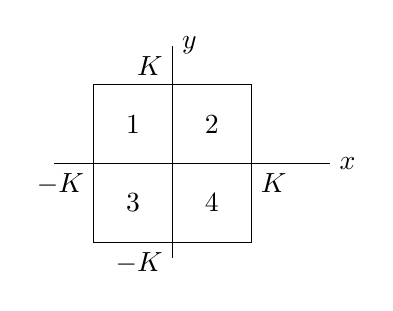
\begin{tikzpicture}
\draw(-1.5,0)--(2,0)node[right]{$x$};
\draw(0,-1.2)--(0,1.5)node[right]{$y$};
\draw(-1,-1) rectangle (1,1);
\draw(0,1)node[above left]{$K$};
\draw(0,-1)node[below left]{$-K$};
\draw(-1,0)node[below left]{$-K$};
\draw(1,0)node[below right]{$K$};
\draw(-0.5,0.5)node{$1$};
\draw(0.5,0.5)node{$2$};
\draw(-0.5,-0.5)node{$3$};
\draw(0.5,-0.5)node{$4$};
\end{tikzpicture}
\caption{مسئلہ \حوالہ{مسئلہ_ترتیب_بلزانو_وائشسٹراس} کا ثبوت}
\label{شکل_مسئلہ_ترتیب_بلزانو_وائشسٹراس}
\end{figure}
\انتہا{ثبوت}
%=======================

ہم اب اس حصے کی مرکزی مسئلہ کو پیش کرنے کے قابل ہیں۔

%==============================
\ابتدا{مسئلہ}\quad \موٹا{(کوشی اصول مرکوزیت برائے ترتیب)}\\

\انتہا{مسئلہ}
%==========================
